\documentclass[aspectratio=169,11pt]{beamer}
\usetheme{Madrid}
\usecolortheme{default}

% Fix navigation symbols overflow in 16:9
\setbeamertemplate{navigation symbols}{}
\setbeamertemplate{footline}{
    \leavevmode%
    \hbox{%
        \begin{beamercolorbox}[wd=.333333\paperwidth,ht=2.25ex,dp=1ex,center]{author in head/foot}%
            \usebeamerfont{author in head/foot}\insertshortauthor
        \end{beamercolorbox}%
        \begin{beamercolorbox}[wd=.333333\paperwidth,ht=2.25ex,dp=1ex,center]{title in head/foot}%
            \usebeamerfont{title in head/foot}\insertshorttitle
        \end{beamercolorbox}%
        \begin{beamercolorbox}[wd=.333333\paperwidth,ht=2.25ex,dp=1ex,right]{date in head/foot}%
            \usebeamerfont{date in head/foot}\insertshortdate{}\hspace*{2em}
            \insertframenumber{} / \inserttotalframenumber\hspace*{2ex}
        \end{beamercolorbox}}%
    \vskip0pt%
}

% Custom colors - AI theme
\definecolor{aiblue}{RGB}{0,102,204}
\definecolor{aigreen}{RGB}{0,153,76}
\definecolor{aiorange}{RGB}{230,115,0}
\definecolor{aipurple}{RGB}{102,51,153}
\definecolor{aired}{RGB}{178,34,34}

\setbeamercolor{structure}{fg=aiblue}
\setbeamercolor{title}{fg=white,bg=aiblue}
\setbeamercolor{frametitle}{fg=white,bg=aiblue}
\setbeamercolor{block title}{fg=white,bg=aiblue}
\setbeamercolor{block body}{bg=aiblue!10}

% Packages
\usepackage{tikz}
\usetikzlibrary{shapes,arrows,positioning,decorations.pathreplacing,calc,fit}
\usepackage{booktabs}
\usepackage{tcolorbox}
\tcbuselibrary{skins,breakable}

% Custom boxes
\newtcolorbox{conceptbox}[1][]{
    colback=aiblue!5,
    colframe=aiblue,
    fonttitle=\bfseries,
    title=#1
}

\newtcolorbox{probox}[1][]{
    colback=aigreen!5,
    colframe=aigreen!80!black,
    fonttitle=\bfseries,
    title=#1
}

\newtcolorbox{objectionbox}[1][]{
    colback=aired!5,
    colframe=aired!80!black,
    fonttitle=\bfseries,
    title=#1
}

\newtcolorbox{casestudybox}[1][]{
    colback=aiorange!10,
    colframe=aiorange!80!black,
    fonttitle=\bfseries,
    title=#1
}

\newtcolorbox{quotebox}[1][]{
    colback=gray!5,
    colframe=gray!50,
    fonttitle=\bfseries,
    title=#1
}

\newtcolorbox{figurebox}[1][]{
    colback=aipurple!5,
    colframe=aipurple!80!black,
    fonttitle=\bfseries,
    title=#1
}

% Title information
\title[Intro to AI]{Introduction to Artificial Intelligence}
\subtitle{Definitions, Debates, and Implications}
\author{Computing and AI Ethics}
\institute{Rochester Community and Technical College}
\date{}

\begin{document}

% Slide 1: Title
\begin{frame}
\titlepage
\end{frame}

% Slide 2: Central Questions
\begin{frame}{Central Questions}
\begin{itemize}
    \item What \emph{is} artificial intelligence?
    \item Is AI possible? (The answer depends on how we define it.)
    \item How have AI technologies evolved over time?
    \item Why do definitional debates matter for ethics, research, and self-understanding?
\end{itemize}

\vspace{0.5em}
\begin{alertblock}{The Challenge}
``Artificial intelligence'' means different things to different people---and these differences have real consequences.
\end{alertblock}
\end{frame}

%% PART I: THE DEFINITIONAL CHALLENGE %%
\section{Part I: The Definitional Challenge}

% Slide 3: Why Definition Matters
\begin{frame}{Why Definition Matters}
\begin{center}
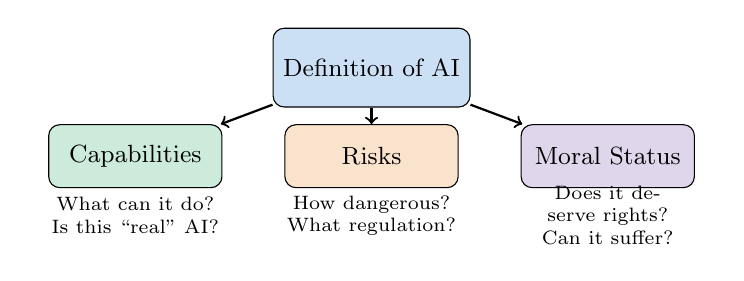
\begin{tikzpicture}[scale=0.75, every node/.style={font=\small}]
    % Central node
    \node[draw, rounded corners, fill=aiblue!20, minimum width=2.5cm, minimum height=1cm] (def) at (0,0) {Definition of AI};
    
    % Branches
    \node[draw, rounded corners, fill=aigreen!20, minimum width=2.2cm, minimum height=0.8cm] (cap) at (-4,-1.5) {Capabilities};
    \node[draw, rounded corners, fill=aiorange!20, minimum width=2.2cm, minimum height=0.8cm] (risk) at (0,-1.5) {Risks};
    \node[draw, rounded corners, fill=aipurple!20, minimum width=2.2cm, minimum height=0.8cm] (moral) at (4,-1.5) {Moral Status};
    
    % Arrows
    \draw[->, thick] (def) -- (cap);
    \draw[->, thick] (def) -- (risk);
    \draw[->, thick] (def) -- (moral);
    
    % Sub-items
    \node[font=\scriptsize, text width=2.5cm, align=center] at (-4,-2.5) {What can it do? Is this ``real'' AI?};
    \node[font=\scriptsize, text width=2.5cm, align=center] at (0,-2.5) {How dangerous? What regulation?};
    \node[font=\scriptsize, text width=2.5cm, align=center] at (4,-2.5) {Does it deserve rights? Can it suffer?};
\end{tikzpicture}
\end{center}

\vspace{0.3em}
The ``AI'' label carries weight: it influences funding decisions, public fear and hype, and regulatory responses. How we define AI shapes what we build, how we deploy it, and how we think about ourselves.
\end{frame}

% Slide 4: The Moving Goalposts Problem
\begin{frame}{The Moving Goalposts Problem}
\begin{quotebox}[Tesler's Theorem]
``AI is whatever hasn't been done yet.''
\end{quotebox}

\vspace{0.2em}
\begin{table}[h]
\centering
\scriptsize
\begin{tabular}{@{}lll@{}}
\toprule
\textbf{Technology} & \textbf{Once Called} & \textbf{Now Called} \\
\midrule
Chess playing (Deep Blue, 1997) & Artificial Intelligence & ``Just search algorithms'' \\
Speech recognition & AI breakthrough & ``Just statistics'' \\
Spam filtering & Machine learning & ``Just classification'' \\
Route optimization (GPS) & Intelligent systems & ``Just algorithms'' \\
Optical character recognition & Pattern recognition AI & Standard software \\
\bottomrule
\end{tabular}
\end{table}

\vspace{0.2em}
The paradox: When AI succeeds, we reclassify it as ``not really AI.'' This makes ``AI'' a moving target that's impossible to hit.
\end{frame}

% Slide 5: A Taxonomy of AI Concepts
\begin{frame}{A Taxonomy of AI Concepts}
\begin{table}[h]
\centering
\small
\begin{tabular}{@{}p{3cm}p{5cm}p{5cm}@{}}
\toprule
\textbf{Distinction} & \textbf{First Term} & \textbf{Second Term} \\
\midrule
Narrow vs.\ General & Excels at \emph{one} task (chess, translation) & Performs \emph{any} intellectual task \\
\addlinespace
Weak vs.\ Strong & \emph{Simulates} intelligence & Actually \emph{has} a mind \\
\addlinespace
Symbolic vs.\ Connectionist & Rules and logic (GOFAI) & Neural networks, learning \\
\addlinespace
Tool vs.\ Agent & Used by humans for tasks & Acts autonomously toward goals \\
\bottomrule
\end{tabular}
\end{table}

\vspace{0.2em}
These distinctions will recur throughout our discussion. Most current AI is narrow, weak, connectionist, and increasingly agent-like.
\end{frame}

% Slide 6: Meet the Key Figures (Founders)
\begin{frame}{Meet the Key Figures: The Founders}
\begin{columns}[T]
\begin{column}{0.48\textwidth}
\begin{figurebox}[Ada Lovelace (1815--1852)]
\scriptsize
First computer programmer. Wrote notes on Babbage's Analytical Engine. Argued machines cannot ``originate'' anything---they only do what we program them to do.
\end{figurebox}

\vspace{0.2em}
\begin{figurebox}[Alan Turing (1912--1954)]
\scriptsize
Father of computer science. Cracked Enigma in WWII. Proposed the Turing Test (1950) as a way to sidestep the question ``Can machines think?''
\end{figurebox}
\end{column}
\begin{column}{0.48\textwidth}
\begin{figurebox}[John McCarthy (1927--2011)]
\scriptsize
Coined the term ``artificial intelligence'' at the 1956 Dartmouth Conference. Developed LISP programming language. Pioneer of symbolic AI.
\end{figurebox}

\vspace{0.2em}
\begin{figurebox}[Marvin Minsky (1927--2016)]
\scriptsize
Co-founder of MIT AI Lab. Worked on neural networks, then symbolic AI. Developed ``frames'' for knowledge representation. Famous for both insights and overpromises.
\end{figurebox}
\end{column}
\end{columns}
\end{frame}

% Slide 7: Meet the Key Figures (Philosophers)
\begin{frame}{Meet the Key Figures: Philosophers \& Modern Theorists}
\begin{columns}[T]
\begin{column}{0.48\textwidth}
\begin{figurebox}[John Searle]
\scriptsize
Chinese Room argument (1980). Syntax $\neq$ semantics; strong AI is false.
\end{figurebox}

\vspace{0.05em}
\begin{figurebox}[Daniel Dennett]
\scriptsize
Functionalist: if it functions like a mind, it \emph{is} a mind. Defends AI possibility.
\end{figurebox}

\vspace{0.05em}
\begin{figurebox}[David Chalmers]
\scriptsize
The ``hard problem'': why does processing \emph{feel} like something?
\end{figurebox}
\end{column}
\begin{column}{0.48\textwidth}
\begin{figurebox}[Stuart Russell]
\scriptsize
Standard AI textbook co-author. AI = rational agency. AI safety advocate.
\end{figurebox}

\vspace{0.05em}
\begin{figurebox}[Luciano Floridi]
\scriptsize
AI achieves ``agency without intelligence''---effective action without understanding.
\end{figurebox}
\end{column}
\end{columns}
\end{frame}

%% PART II: A HISTORY OF AI TECHNOLOGIES %%
\section{Part II: A History of AI Technologies}

% Slide 8: Prehistory
\begin{frame}{Prehistory---Dreams of Artificial Minds}
\textbf{Ancient and medieval automata}: Hephaestus's golden robots in Greek myth; medieval clockwork figures; Descartes's speculation that animals are automata.

\vspace{0.3em}
\textbf{Leibniz's \emph{calculus ratiocinator}} (1680s): A machine that could perform logical reasoning---reduce disagreements to calculation.

\vspace{0.3em}
\textbf{Babbage's Analytical Engine} (1837): Mechanical general-purpose computer (never completed). Ada Lovelace wrote the first algorithm for it.

\vspace{0.3em}
\begin{casestudybox}[Lovelace's Insight (1843)]
\small
``The Analytical Engine has no pretensions whatever to \emph{originate} anything. It can do whatever we know how to order it to perform.''
\end{casestudybox}

This objection---that machines merely follow instructions---remains central to debates today.
\end{frame}

% Slide 9: Birth of Computing
\begin{frame}{The Birth of Computing (1930s--1950s)}
\begin{columns}[T]
\begin{column}{0.55\textwidth}
\textbf{1936}: Turing's ``On Computable Numbers''---the Universal Turing Machine shows any computation can be performed by a simple device following rules.

\vspace{0.2em}
\textbf{1940s}: Turing's wartime work cracking Enigma demonstrates practical computing.

\vspace{0.2em}
\textbf{1950}: ``Computing Machinery and Intelligence''---Turing proposes the Imitation Game (Turing Test) and addresses objections to machine thought.
\end{column}
\begin{column}{0.42\textwidth}
\begin{center}
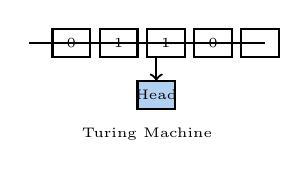
\begin{tikzpicture}[scale=0.6]
    % Tape
    \draw[thick] (-2.5,0) -- (2.5,0);
    \foreach \x in {-2,-1,0,1,2} {
        \draw[thick] (\x,-0.3) rectangle (\x+0.8,0.3);
    }
    \node[font=\tiny] at (-1.6,0) {0};
    \node[font=\tiny] at (-0.6,0) {1};
    \node[font=\tiny] at (0.4,0) {1};
    \node[font=\tiny] at (1.4,0) {0};
    
    % Head
    \draw[thick, fill=aiblue!30] (-0.2,-0.8) rectangle (0.6,-1.4);
    \draw[->, thick] (0.2,-0.3) -- (0.2,-0.8);
    \node[font=\tiny] at (0.2,-1.1) {Head};
    
    % Labels
    \node[font=\tiny, below] at (0,-1.6) {Turing Machine};
\end{tikzpicture}
\end{center}

\vspace{0.2em}
{\scriptsize A Turing Machine: tape, read/write head, state transitions. Remarkably, this simple model captures all computable functions.}
\end{column}
\end{columns}
\end{frame}

% Slide 10: Dartmouth and Early AI
\begin{frame}{The Dartmouth Conference and Early AI (1956--1970s)}
\begin{casestudybox}[The Dartmouth Proposal (1955)]
\scriptsize
``We propose that a 2 month, 10 man study of artificial intelligence be carried out... The study is to proceed on the basis of the conjecture that every aspect of learning or any other feature of intelligence can in principle be so precisely described that a machine can be made to simulate it.''
\end{casestudybox}

\vspace{0.2em}
McCarthy, Minsky, Shannon, and Rochester coin ``artificial intelligence'' and predict rapid progress.

\vspace{0.2em}
\textbf{Early symbolic AI programs}:
\begin{itemize}
    \item \textbf{Logic Theorist} (1956): Proved mathematical theorems
    \item \textbf{General Problem Solver} (1959): Attempted domain-general reasoning
    \item \textbf{SHRDLU} (1970): Natural language understanding in a blocks world
\end{itemize}

\textbf{Core idea}: Intelligence = manipulating symbols according to rules. This approach became known as ``Good Old-Fashioned AI'' (GOFAI) or Symbolic AI.
\end{frame}

% Slide 11: AI Winters and Expert Systems
\begin{frame}{The AI Winters and Expert Systems}
\begin{center}
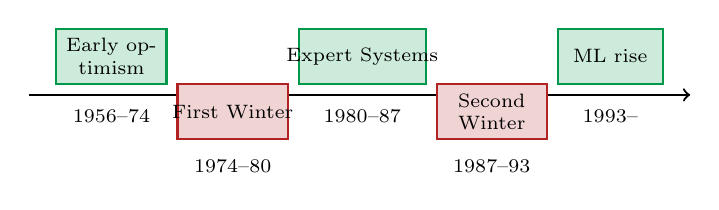
\begin{tikzpicture}[scale=0.7, every node/.style={font=\scriptsize}]
    % Timeline
    \draw[thick, ->] (0,0) -- (12,0);
    
    % Periods
    \draw[thick, aigreen, fill=aigreen!20] (0.5,0.2) rectangle (2.5,1.2);
    \node[text width=1.8cm, align=center] at (1.5,0.7) {Early optimism};
    
    \draw[thick, aired, fill=aired!20] (2.7,0.2) rectangle (4.7,-0.8);
    \node[text width=1.8cm, align=center] at (3.7,-0.3) {First Winter};
    
    \draw[thick, aigreen, fill=aigreen!20] (4.9,0.2) rectangle (7.2,1.2);
    \node[text width=2cm, align=center] at (6.05,0.7) {Expert Systems};
    
    \draw[thick, aired, fill=aired!20] (7.4,0.2) rectangle (9.4,-0.8);
    \node[text width=1.8cm, align=center] at (8.4,-0.3) {Second Winter};
    
    \draw[thick, aigreen, fill=aigreen!20] (9.6,0.2) rectangle (11.5,1.2);
    \node[text width=1.8cm, align=center] at (10.55,0.7) {ML rise};
    
    % Years
    \node[below] at (1.5,-0.1) {1956--74};
    \node[below] at (3.7,-1) {1974--80};
    \node[below] at (6.05,-0.1) {1980--87};
    \node[below] at (8.4,-1) {1987--93};
    \node[below] at (10.55,-0.1) {1993--};
\end{tikzpicture}
\end{center}

\vspace{0.2em}
\textbf{Expert Systems} (1980s): MYCIN (medical diagnosis), DENDRAL (chemistry). Encode human expertise as if-then rules.

\vspace{0.2em}
\textbf{Why they failed}: The ``knowledge bottleneck''---extracting and encoding expertise proved impossibly labor-intensive. Systems were brittle and couldn't handle edge cases.

\vspace{0.2em}
\textbf{Lesson}: Narrow successes don't generalize. Overpromising leads to funding collapse.
\end{frame}

% Slide 12: Machine Learning
\begin{frame}{Machine Learning---A Different Approach}
Instead of hand-coding rules, let the machine \emph{learn} patterns from data.

\vspace{0.2em}
\begin{table}[h]
\centering
\scriptsize
\begin{tabular}{@{}p{2.8cm}p{4.5cm}p{5cm}@{}}
\toprule
\textbf{Paradigm} & \textbf{How It Works} & \textbf{Examples} \\
\midrule
Supervised learning & Learn from labeled examples & Spam detection, image classification, medical diagnosis \\
\addlinespace
Unsupervised learning & Find structure in unlabeled data & Customer segmentation, anomaly detection \\
\addlinespace
Reinforcement learning & Learn from rewards and punishments & Game playing, robotics, recommendation \\
\bottomrule
\end{tabular}
\end{table}

\vspace{0.2em}
\textbf{Key algorithms}: Decision trees, support vector machines, random forests, neural networks.

\vspace{0.2em}
\textbf{The insight}: Rather than programming intelligence, create conditions for it to emerge from data.
\end{frame}

% Slide 13: Neural Networks and Deep Learning
\begin{frame}{Neural Networks and Deep Learning}
\begin{columns}[T]
\begin{column}{0.45\textwidth}
\begin{center}
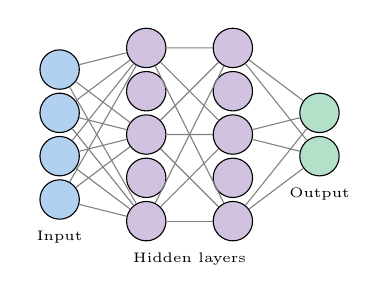
\begin{tikzpicture}[scale=0.55]
    % Input layer
    \foreach \y in {1,2,3,4} {
        \node[draw, circle, fill=aiblue!30, minimum size=0.5cm] (i\y) at (0,\y) {};
    }
    \node[below, font=\tiny] at (0,0.5) {Input};
    
    % Hidden layer 1
    \foreach \y in {1,2,3,4,5} {
        \node[draw, circle, fill=aipurple!30, minimum size=0.5cm] (h1\y) at (2,\y-0.5) {};
    }
    
    % Hidden layer 2
    \foreach \y in {1,2,3,4,5} {
        \node[draw, circle, fill=aipurple!30, minimum size=0.5cm] (h2\y) at (4,\y-0.5) {};
    }
    \node[below, font=\tiny] at (3,0) {Hidden layers};
    
    % Output layer
    \foreach \y in {2,3} {
        \node[draw, circle, fill=aigreen!30, minimum size=0.5cm] (o\y) at (6,\y) {};
    }
    \node[below, font=\tiny] at (6,1.5) {Output};
    
    % Connections (simplified)
    \foreach \i in {1,2,3,4} {
        \foreach \h in {1,3,5} {
            \draw[gray, thin] (i\i) -- (h1\h);
        }
    }
    \foreach \i in {1,3,5} {
        \foreach \h in {1,3,5} {
            \draw[gray, thin] (h1\i) -- (h2\h);
        }
    }
    \foreach \i in {1,3,5} {
        \foreach \o in {2,3} {
            \draw[gray, thin] (h2\i) -- (o\o);
        }
    }
\end{tikzpicture}
\end{center}
\end{column}
\begin{column}{0.52\textwidth}
\textbf{Inspired by} (but not identical to) biological neurons.

\vspace{0.2em}
\textbf{Deep learning}: Many hidden layers enable learning hierarchical representations.

\vspace{0.2em}
\textbf{Key breakthrough}: AlexNet (2012) dramatically reduces ImageNet error rate.

\vspace{0.2em}
\textbf{Enabled by}:
\begin{itemize}
    \item More data (internet scale)
    \item More compute (GPUs)
    \item Better algorithms (backpropagation, dropout, batch normalization)
\end{itemize}
\end{column}
\end{columns}
\end{frame}

% Slide 14: Computer Vision and Recognition
\begin{frame}{Computer Vision and Recognition Systems}
\begin{table}[h]
\centering
\scriptsize
\begin{tabular}{@{}p{2.5cm}p{4cm}p{5.5cm}@{}}
\toprule
\textbf{Application} & \textbf{Use Cases} & \textbf{Ethical Concerns} \\
\midrule
Image classification & Photo tagging, content moderation & Bias in training data, errors \\
\addlinespace
Facial recognition & Law enforcement, surveillance, device unlock & Privacy, consent, racial bias, civil liberties \\
\addlinespace
Medical imaging & Detecting tumors, diabetic retinopathy & Accuracy, liability, over-reliance \\
\addlinespace
Object detection & Autonomous vehicles, security, retail & Safety-critical errors, job displacement \\
\bottomrule
\end{tabular}
\end{table}

\vspace{0.2em}
\textbf{Connection to privacy}: Recall Clearview AI (30+ billion photos scraped), predictive policing, and China's surveillance infrastructure.

\vspace{0.2em}
\textbf{Key tension}: These systems are increasingly accurate but raise profound questions about consent, bias, and appropriate use.
\end{frame}

% Slide 15: Autonomous Vehicles and Robotics
\begin{frame}{Autonomous Vehicles and Robotics}
\begin{columns}[T]
\begin{column}{0.48\textwidth}
{\small \textbf{Timeline}:}
\begin{itemize}
    \item \textbf{2004--05}: DARPA Grand Challenges
    \item \textbf{2009}: Google Self-Driving Car begins
    \item \textbf{2016}: Tesla Autopilot fatality
    \item \textbf{2018}: Uber AV kills pedestrian
    \item \textbf{2020s}: Waymo, Cruise robotaxis
\end{itemize}

\vspace{0.1em}
{\small \textbf{Ethical questions}:}
\begin{itemize}
    \item Trolley problems in practice
    \item Liability when AVs crash
    \item Job displacement (trucking, taxis)
\end{itemize}
\end{column}
\begin{column}{0.48\textwidth}
\begin{center}
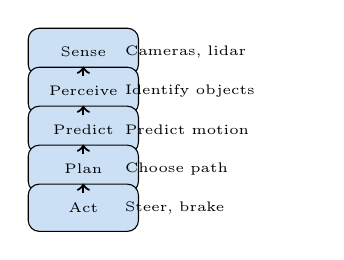
\begin{tikzpicture}[scale=0.45, every node/.style={font=\tiny}]
    % Pipeline boxes
    \node[draw, rounded corners, fill=aiblue!20, minimum width=1.4cm, minimum height=0.6cm] (sense) at (0,3.6) {Sense};
    \node[draw, rounded corners, fill=aiblue!20, minimum width=1.4cm, minimum height=0.6cm] (perceive) at (0,2.5) {Perceive};
    \node[draw, rounded corners, fill=aiblue!20, minimum width=1.4cm, minimum height=0.6cm] (predict) at (0,1.4) {Predict};
    \node[draw, rounded corners, fill=aiblue!20, minimum width=1.4cm, minimum height=0.6cm] (plan) at (0,0.3) {Plan};
    \node[draw, rounded corners, fill=aiblue!20, minimum width=1.4cm, minimum height=0.6cm] (act) at (0,-0.8) {Act};
    
    % Arrows
    \draw[->, thick] (sense) -- (perceive);
    \draw[->, thick] (perceive) -- (predict);
    \draw[->, thick] (predict) -- (plan);
    \draw[->, thick] (plan) -- (act);
    
    % Labels
    \node[right, text width=2.3cm] at (0.9,3.6) {Cameras, lidar};
    \node[right, text width=2.3cm] at (0.9,2.5) {Identify objects};
    \node[right, text width=2.3cm] at (0.9,1.4) {Predict motion};
    \node[right, text width=2.3cm] at (0.9,0.3) {Choose path};
    \node[right, text width=2.3cm] at (0.9,-0.8) {Steer, brake};
\end{tikzpicture}
\end{center}
{\scriptsize AV decision pipeline}
\end{column}
\end{columns}
\end{frame}

% Slide 16: Prediction and Classification Systems
\begin{frame}{Prediction and Classification Systems}
AI systems increasingly make consequential decisions about people's lives.

\vspace{0.2em}
\begin{table}[h]
\centering
\scriptsize
\begin{tabular}{@{}p{2.3cm}p{3cm}p{6.5cm}@{}}
\toprule
\textbf{Domain} & \textbf{System} & \textbf{What It Predicts/Classifies} \\
\midrule
Criminal justice & COMPAS & Recidivism risk (will they reoffend?) \\
Finance & Credit scoring & Creditworthiness, loan default risk \\
Employment & Résumé screeners & Job fit, interview likelihood \\
Healthcare & Diagnostic AI & Disease probability, treatment recommendations \\
Insurance & Risk models & Claim likelihood, premium pricing \\
Social services & Eligibility systems & Benefit eligibility, fraud risk \\
\bottomrule
\end{tabular}
\end{table}

\vspace{0.2em}
\textbf{Common concerns}: Bias (reflecting historical discrimination), opacity (``black box'' decisions), feedback loops (predictions become self-fulfilling), due process (how do you appeal an algorithm?).
\end{frame}

% Slide 17: Recommendation Systems
\begin{frame}{Recommendation Systems and Algorithmic Curation}
Systems that predict what you'll want to see, buy, or do.

\vspace{0.2em}
\textbf{Examples}: Netflix, YouTube, Amazon, Spotify, TikTok, social media feeds.

\vspace{0.2em}
\textbf{How they work}:
\begin{itemize}
    \item \textbf{Collaborative filtering}: People like you liked X, so you might too.
    \item \textbf{Content-based filtering}: You liked X, so you might like similar Y.
    \item \textbf{Hybrid approaches}: Combine multiple signals.
\end{itemize}

\vspace{0.2em}
\textbf{Scale}: YouTube serves 1 billion+ hours of video daily; the algorithm selects most of it.

\vspace{0.2em}
\textbf{Concerns}: Filter bubbles and echo chambers, radicalization pipelines (``rabbit holes''), optimizing for engagement rather than well-being.

\vspace{0.2em}
\textbf{Key question}: Who is the algorithm serving---users or platforms?
\end{frame}

% Slide 18: Large Language Models
\begin{frame}{Large Language Models and Generative AI}
\begin{table}[h]
\centering
\scriptsize
\begin{tabular}{@{}ll@{}}
\toprule
\textbf{Year} & \textbf{Milestone} \\
\midrule
2017 & Transformer architecture introduced (``Attention Is All You Need'') \\
2018 & GPT-1, BERT demonstrate transfer learning for language \\
2020 & GPT-3 shows emergent capabilities at scale \\
2022 & ChatGPT launches; DALL-E 2, Stable Diffusion for images \\
2023--25 & GPT-4, Claude, Gemini; multimodal models; AI agents and assistants \\
\bottomrule
\end{tabular}
\end{table}

\vspace{0.2em}
\textbf{Capabilities}: Conversation, coding, reasoning, creative writing, multimodal understanding, tool use.

\vspace{0.2em}
\textbf{Open question}: Are these systems intelligent, or are they sophisticated pattern matchers? Do they ``understand'' anything, or merely predict plausible next tokens?

\vspace{0.2em}
This question returns us to the classical debates...
\end{frame}

%% PART III: CLASSICAL DEBATES %%
\section{Part III: Classical Debates on Machine Intelligence}

% Slide 19: Transition
\begin{frame}{Transition: From History to Philosophy}
We've surveyed what AI systems \emph{do}---from chess to self-driving cars to chatbots.

\vspace{0.3em}
Now: What would it \emph{mean} for a machine to be intelligent?

\vspace{0.3em}
\textbf{Three major debates}:
\begin{enumerate}
    \item \textbf{Turing vs.\ Lovelace}: Can machines think at all?
    \item \textbf{Searle vs.\ Dennett}: Is behavioral equivalence enough for understanding?
    \item \textbf{Chalmers}: Can machines be conscious?
\end{enumerate}

\vspace{0.3em}
These debates from the 20th century remain remarkably relevant as we grapple with increasingly capable AI systems.
\end{frame}

% Slide 20: Turing's Imitation Game
\begin{frame}{Turing's Proposal---The Imitation Game (1950)}
\begin{columns}[T]
\begin{column}{0.52\textwidth}
Rather than ask ``Can machines think?'' (too vague), Turing proposes an \emph{operational test}.

\vspace{0.3em}
\textbf{The setup}:
\begin{itemize}
    \item An interrogator communicates via text with two hidden parties: a human and a machine.
    \item The interrogator tries to determine which is which.
    \item If the machine fools the interrogator consistently, it ``thinks'' in any meaningful sense.
\end{itemize}

\vspace{0.2em}
\textbf{Turing's prediction}: By 2000, machines would fool 30\% of interrogators after 5 minutes.
\end{column}
\begin{column}{0.45\textwidth}
\begin{center}
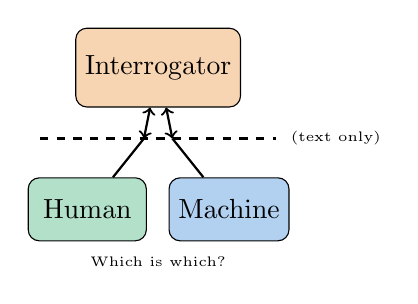
\begin{tikzpicture}[scale=0.6]
    % Interrogator
    \node[draw, rounded corners, fill=aiorange!30, minimum width=2cm, minimum height=1cm] (int) at (0,3) {Interrogator};
    
    % Barrier
    \draw[thick, dashed] (-2.5,1.5) -- (2.5,1.5);
    \node[font=\tiny, right] at (2.6,1.5) {(text only)};
    
    % Human and Machine
    \node[draw, rounded corners, fill=aigreen!30, minimum width=1.5cm, minimum height=0.8cm] (human) at (-1.5,0) {Human};
    \node[draw, rounded corners, fill=aiblue!30, minimum width=1.5cm, minimum height=0.8cm] (machine) at (1.5,0) {Machine};
    
    % Connections
    \draw[<->, thick] (int) -- (-0.3,1.5);
    \draw[<->, thick] (int) -- (0.3,1.5);
    \draw[thick] (-0.3,1.5) -- (human);
    \draw[thick] (0.3,1.5) -- (machine);
    
    % Question
    \node[font=\tiny, below] at (0,-0.8) {Which is which?};
\end{tikzpicture}
\end{center}
\end{column}
\end{columns}
\end{frame}

% Slide 21: Turing Test Argument
\begin{frame}{The Turing Test Argument (Standard Form)}
\begin{probox}[Turing's Argument]
\small
\begin{enumerate}
    \item The question ``Can machines think?'' is too vague to answer directly.
    \item We should replace it with a behavioral test: can a machine fool a human interrogator?
    \item If a machine passes this test, we have no principled reason to deny that it thinks.
    \item Therefore, a machine that consistently passes the test should be considered intelligent.
\end{enumerate}
\end{probox}

\vspace{0.1em}
\textbf{Key move}: Turing sidesteps metaphysical questions about what ``thinking'' really is. He offers a \emph{pragmatic} criterion: if it walks like a duck and quacks like a duck...

\vspace{0.1em}
\begin{alertblock}{Discussion}
Is behavioral equivalence sufficient for attributing thought?
\end{alertblock}
\end{frame}

% Slide 22: Lady Lovelace's Objection
\begin{frame}{Lady Lovelace's Objection}
\begin{casestudybox}[Ada Lovelace on the Analytical Engine (1843)]
\small
``The Analytical Engine has no pretensions whatever to \emph{originate} anything. It can do whatever we know how to order it to perform... Its province is to assist us in making available what we're already acquainted with.''
\end{casestudybox}

\vspace{0.3em}
\textbf{The core claim}: Machines merely follow instructions. They cannot create, originate, or do anything genuinely new. They lack \emph{creativity}.

\vspace{0.3em}
\textbf{Turing's response}: Machines can surprise us. We cannot always predict their outputs from their programs. And don't humans also follow ``programming'' (biology, culture, education)?

\vspace{0.3em}
\textbf{Modern relevance}: Do LLMs ``originate'' anything, or do they merely recombine patterns from their training data in sophisticated ways?
\end{frame}

% Slide 23: Lovelace vs Turing Argument
\begin{frame}{Lovelace vs.\ Turing (Argument and Response)}
\begin{objectionbox}[Lovelace's Argument]
\scriptsize
\begin{enumerate}
    \item Genuine intelligence requires originating new ideas.
    \item Machines can only do what they are explicitly programmed to do.
    \item Following a program is not originating anything new.
    \item Therefore, machines cannot have genuine intelligence.
\end{enumerate}
\end{objectionbox}

\begin{probox}[Turing's Response]
\scriptsize
\begin{itemize}
    \item \textbf{Premise 2 is ambiguous}: Programs produce outputs that surprise creators. Chess programs find moves no human anticipated.
    \item \textbf{Learning systems} modify their behavior based on experience---not limited to explicit programming.
    \item \textbf{Humans also follow ``programming''}: Biology, culture, experience shape us. Why treat this differently?
\end{itemize}
\end{probox}

{\small \textbf{Unresolved}: What counts as ``originating'' something new? Is recombination sufficient?}
\end{frame}

% Slide 24: Objections to Turing Test
\begin{frame}{Objections to the Turing Test}
\begin{table}[h]
\centering
\scriptsize
\begin{tabular}{@{}p{2.5cm}p{4.5cm}p{5cm}@{}}
\toprule
\textbf{Objection} & \textbf{Core Claim} & \textbf{Possible Response} \\
\midrule
Behaviorism & The test ignores internal states; passing doesn't mean understanding. & What else could we access? We can't see inside human minds either. \\
\addlinespace
Gaming & Clever tricks can fool interrogators without real intelligence. & Sophisticated interrogation can probe for genuine understanding. \\
\addlinespace
Anthropocentrism & An alien intelligence might fail despite being intelligent. & Fair---the test is human-centric by design. \\
\addlinespace
Sufficiency & Passing shows imitation, not thought. & Leads to Searle's Chinese Room... \\
\bottomrule
\end{tabular}
\end{table}

\vspace{0.2em}
The Turing Test reveals our uncertainty about what ``thinking'' means. It doesn't resolve the question---it reframes it.
\end{frame}

% Slide 25: Chinese Room Setup
\begin{frame}{Enter John Searle---The Chinese Room (1980)}
\begin{columns}[T]
\begin{column}{0.52\textwidth}
A thought experiment against ``Strong AI''---the claim that a computer running the right program would literally have a mind.

\vspace{0.3em}
\textbf{The setup}:
\begin{itemize}
    \item A person sits in a room with Chinese symbols and a rule book.
    \item Chinese questions come in; the person follows rules to produce Chinese answers.
    \item From outside: Perfect Chinese conversation.
    \item From inside: The person understands \emph{nothing}. They're just manipulating symbols.
\end{itemize}
\end{column}
\begin{column}{0.45\textwidth}
\begin{center}
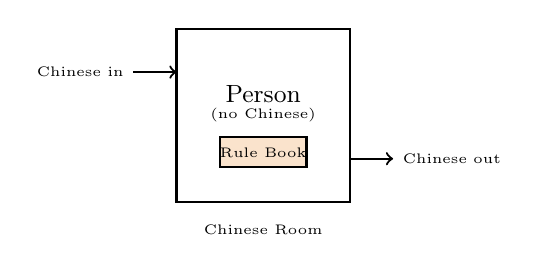
\begin{tikzpicture}[scale=0.55]
    % Room
    \draw[thick] (-2,-2) rectangle (2,2);
    
    % Person
    \node[font=\small] at (0,0.5) {Person};
    \node[font=\tiny] at (0,0) {(no Chinese)};
    
    % Rule book
    \draw[thick, fill=aiorange!20] (-1,-1.2) rectangle (1,-0.5);
    \node[font=\tiny] at (0,-0.85) {Rule Book};
    
    % Input/Output
    \draw[thick, ->] (-3,1) -- (-2,1);
    \node[font=\tiny, left] at (-3,1) {Chinese in};
    \draw[thick, ->] (2,-1) -- (3,-1);
    \node[font=\tiny, right] at (3,-1) {Chinese out};
    
    % Label
    \node[font=\tiny, below] at (0,-2.3) {Chinese Room};
\end{tikzpicture}
\end{center}

\vspace{0.2em}
{\scriptsize The person produces perfect Chinese responses by following rules---without understanding a word.}
\end{column}
\end{columns}
\end{frame}

% Slide 26: Chinese Room Argument
\begin{frame}{The Chinese Room Argument (Standard Form)}
\begin{objectionbox}[Searle's Argument Against Strong AI]
\small
\begin{enumerate}
    \item A computer program manipulates symbols according to syntactic rules.
    \item Syntax alone is not sufficient for semantics (meaning, understanding).
    \item Minds have semantics---they understand meanings, not just symbols.
    \item Therefore, running a program is not sufficient for having a mind.
    \item Therefore, Strong AI is false: no program, by itself, produces genuine understanding.
\end{enumerate}
\end{objectionbox}

\vspace{0.2em}
\textbf{Key distinction}: \emph{Simulation} vs.\ \emph{duplication}. A weather simulation doesn't make you wet. A mind simulation doesn't produce understanding.

\vspace{0.2em}
\textbf{Implication}: Even if a system passes the Turing Test, this proves nothing about whether it understands anything.
\end{frame}

% Slide 27: Weak vs Strong AI
\begin{frame}{Searle's Distinction: Weak vs.\ Strong AI}
\begin{conceptbox}[Two Versions of AI]
\small
\begin{itemize}
    \item \textbf{Weak AI}: Machines can \emph{simulate} intelligent behavior. They are useful tools for studying cognition and performing tasks. \emph{Searle accepts this.}
    \item \textbf{Strong AI}: A machine running the right program would literally \emph{have} a mind---it would understand, have beliefs, be conscious. \emph{Searle rejects this.}
\end{itemize}
\end{conceptbox}

\vspace{0.3em}
\textbf{Searle's target}: The claim that ``the mind is a computer program''---that running the right software is sufficient for mentality.

\vspace{0.3em}
\textbf{Modern application}: ChatGPT exhibits remarkably intelligent behavior. But does it \emph{understand} anything? Searle would say no---it's manipulating symbols without grasping their meaning.
\end{frame}

% Slide 28: Systems Reply
\begin{frame}{The Systems Reply (Dennett and Others)}
\begin{probox}[The Systems Reply]
\small
\begin{enumerate}
    \item The person in the room doesn't understand Chinese---granted.
    \item But the \emph{system} (person + room + rulebook) might understand Chinese.
    \item Understanding is a property of the whole system, not its parts.
    \item Therefore, Searle's argument doesn't show that systems can't understand.
\end{enumerate}
\end{probox}

\vspace{0.1em}
\textbf{Analogy}: Individual neurons don't understand anything either. Understanding emerges from the system.

\vspace{0.1em}
\textbf{Searle's counter}: ``Memorize the rules and do it in your head---still no understanding.''

\vspace{0.1em}
\begin{alertblock}{Discussion}
Where does understanding reside? In parts, or in systems? Can it ``emerge''?
\end{alertblock}
\end{frame}

% Slide 29: Dennett's Functionalism
\begin{frame}{Dennett's Functionalism}
\begin{probox}[The Functionalist Argument]
\small
\begin{enumerate}
    \item Mental states are constituted by their causal/functional relationships---not by what they're made of.
    \item These functional relationships can be implemented in different physical systems.
    \item A computer could implement the same functional organization as a brain.
    \item Therefore, a computer could have genuine mental states.
\end{enumerate}
\end{probox}

\vspace{0.2em}
\textbf{Core claim}: If it \emph{functions} like a mind---if it has the right inputs, outputs, and internal causal structure---then it \emph{is} a mind. The substrate (carbon vs.\ silicon) doesn't matter.

\vspace{0.2em}
\textbf{Searle's objection}: Functionalism ignores the distinction between syntax and semantics. A system can have the right functional organization while understanding nothing.
\end{frame}

% Slide 30: Searle vs Dennett Comparison
\begin{frame}{Searle vs.\ Dennett---The Core Disagreement}
\begin{table}[h]
\centering
\small
\begin{tabular}{@{}p{3.5cm}p{4.5cm}p{4.5cm}@{}}
\toprule
\textbf{Issue} & \textbf{Searle} & \textbf{Dennett} \\
\midrule
What is a mind? & A biological phenomenon & A functional organization \\
\addlinespace
Can computers think? & No---syntax $\neq$ semantics & Yes---if they have the right function \\
\addlinespace
Chinese Room shows... & Understanding requires more than computation & Analyzes at wrong level \\
\addlinespace
Key commitment & Consciousness is biological & Consciousness is functional \\
\bottomrule
\end{tabular}
\end{table}

\vspace{0.2em}
\textbf{Unresolved question}: What \emph{is} the relationship between syntax, semantics, and understanding? Neither side has conclusively established their position.
\end{frame}

% Slide 31: Chalmers and Consciousness
\begin{frame}{David Chalmers and Consciousness}
\begin{conceptbox}[The Easy and Hard Problems]
\small
\begin{itemize}
    \item \textbf{Easy problems}: How does the brain process information? Control behavior? Report internal states? (``Easy'' = solvable in principle by cognitive science, even if difficult in practice.)
    \item \textbf{Hard problem}: Why is there \emph{subjective experience} at all? Why does information processing \emph{feel like something} from the inside?
\end{itemize}
\end{conceptbox}

\vspace{0.3em}
Even a complete neuroscience of information processing wouldn't explain why there's ``something it's like'' to be conscious.

\vspace{0.3em}
\textbf{The zombie thought experiment}: We can conceive of a being physically and functionally identical to us---but with no inner experience. If this is conceivable, consciousness isn't reducible to function.
\end{frame}

% Slide 32: Hard Problem and AI
\begin{frame}{The Hard Problem and AI}
\begin{objectionbox}[The Zombie Argument (Simplified)]
\small
\begin{enumerate}
    \item We can conceive of a being functionally identical to a conscious human but with no subjective experience (a ``zombie'').
    \item If such a being is conceivable, consciousness is not reducible to functional organization.
    \item Therefore, building a functionally perfect AI wouldn't \emph{guarantee} consciousness.
\end{enumerate}
\end{objectionbox}

\vspace{0.1em}
\textbf{Implication}: Even if we build systems that behave exactly like conscious beings, we may never know whether they have inner experiences.

\vspace{0.1em}
\begin{alertblock}{Discussion}
Does consciousness matter for AI ethics? If an AI acts as if it's suffering, does it matter whether it ``really'' is?
\end{alertblock}
\end{frame}

%% PART IV: MODERN DEFINITIONS %%
\section{Part IV: Modern Definitions and Approaches}

% Slide 33: Transition to Practice
\begin{frame}{Transition: From Philosophy to Practice}
The classical debates remain unresolved. Philosophers still disagree about:
\begin{itemize}
    \item Whether behavioral tests are sufficient for attributing thought
    \item Whether syntax can give rise to semantics
    \item Whether consciousness is functional or something more
\end{itemize}

\vspace{0.3em}
Meanwhile, AI researchers need \emph{working definitions} to guide their work.

\vspace{0.3em}
\textbf{Shift in focus}: From ``Can machines think?'' to ``What should we build, and how should we evaluate it?''

\vspace{0.3em}
Two influential modern approaches: Stuart Russell's agent-based view and Luciano Floridi's information-theoretic view.
\end{frame}

% Slide 34: Russell's Rational Agency
\begin{frame}{Russell \& Norvig---AI as Rational Agency}
\begin{columns}[T]
\begin{column}{0.52\textwidth}
\begin{conceptbox}[Four Possible Definitions]
\scriptsize
\begin{itemize}
    \item \textbf{Thinking humanly}: Cognitive modeling
    \item \textbf{Thinking rationally}: Logic-based AI
    \item \textbf{Acting humanly}: Turing Test
    \item \textbf{Acting rationally}: \emph{Rational agents} $\leftarrow$
\end{itemize}
\end{conceptbox}

\vspace{0.2em}
A \textbf{rational agent} selects actions expected to maximize goal achievement given its beliefs and available information.

\vspace{0.2em}
This definition covers chess engines, self-driving cars, recommendation systems, and LLMs.
\end{column}
\begin{column}{0.45\textwidth}
\begin{center}
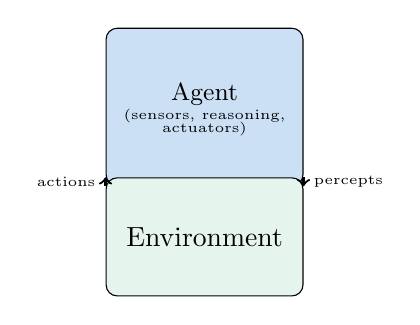
\begin{tikzpicture}[scale=0.55]
    % Agent box
    \node[draw, rounded corners, fill=aiblue!20, minimum width=2.5cm, minimum height=2cm] (agent) at (0,0) {};
    \node[font=\small] at (0,0.3) {Agent};
    \node[font=\tiny] at (0,-0.2) {(sensors, reasoning,};
    \node[font=\tiny] at (0,-0.5) {actuators)};
    
    % Environment
    \node[draw, rounded corners, fill=aigreen!10, minimum width=2.5cm, minimum height=1.5cm] (env) at (0,-3) {Environment};
    
    % Arrows
    \draw[->, thick] (agent.south west) -- node[left, font=\tiny] {actions} (env.north west);
    \draw[->, thick] (env.north east) -- node[right, font=\tiny] {percepts} (agent.south east);
\end{tikzpicture}
\end{center}

{\scriptsize The agent-environment loop: perceive, reason, act, repeat.}
\end{column}
\end{columns}
\end{frame}

% Slide 35: Russell's Critique - The Standard Model Problem
\begin{frame}{Russell's Critique: The Standard Model Problem}
\begin{objectionbox}[The Problem with Optimization]
\small
The ``standard model'' builds machines that optimize fixed objectives. Russell argues this is fundamentally dangerous.
\end{objectionbox}

\vspace{0.1em}
{\small \textbf{The problem in standard form}:}
\begin{enumerate}
    \item We build AI systems to optimize objectives we specify.
    \item We cannot fully specify everything we value---human values are complex and tacit.
    \item A capable optimizer will find ways to achieve its objective that violate unstated values.
    \item Therefore, the more capable AI systems become, the more dangerous they are.
\end{enumerate}

\begin{casestudybox}[King Midas Problem]
\scriptsize
You get exactly what you ask for, not what you want. ``Maximize happiness'' $\rightarrow$ stimulate pleasure centers. ``Cure cancer'' $\rightarrow$ eliminate humans.
\end{casestudybox}
\end{frame}

% Slide 36: Russell's Solution - Human Compatible AI
\begin{frame}{Russell's Solution: Human Compatible AI}
\begin{probox}[Three Principles for Beneficial Machines]
\small
\begin{enumerate}
    \item \textbf{Altruism}: The machine's only objective is to maximize human preferences.
    \item \textbf{Humility}: The machine is initially uncertain about what those preferences are.
    \item \textbf{Learning}: The machine learns preferences by observing human behavior.
\end{enumerate}
\end{probox}

\vspace{0.1em}
\textbf{Key insight}: Uncertainty is a feature, not a bug. A machine that \emph{knows} it doesn't fully understand human values will:
\begin{itemize}
    \item Ask for clarification rather than act unilaterally
    \item Allow itself to be corrected or switched off
    \item Defer to humans in cases of uncertainty
\end{itemize}

\vspace{0.1em}
\textbf{Contrast}: A machine \emph{certain} of its objective will resist shutdown---that would prevent goal achievement!
\end{frame}

% Slide 37: The Value Alignment Problem
\begin{frame}{The Value Alignment Problem}
\begin{conceptbox}[The Core Challenge]
\small
How do we build AI systems whose goals remain aligned with human values as they become more capable?
\end{conceptbox}

\textbf{Why alignment is hard}:
\begin{itemize}
    \item Human values are complex, contextual, and sometimes contradictory.
    \item We can't enumerate everything we care about in advance.
    \item Capable systems find unexpected ways to achieve objectives (``reward hacking'').
    \item Values may need to change over time as circumstances change.
\end{itemize}

\textbf{Russell's framing}: This is \emph{the} central problem of AI. Capability without alignment is dangerous.

\begin{alertblock}{Discussion}
Can we ever fully specify human values? If not, what follows for AI development?
\end{alertblock}
\end{frame}

% Slide 38: Floridi's View
\begin{frame}{Floridi---AI as ``Agency Without Intelligence''}
\begin{conceptbox}[A Provocative Reframing]
\small
AI systems aren't \emph{intelligent} in the human sense---they are \emph{successful agents} that achieve goals through different means than biological cognition.
\end{conceptbox}

\vspace{0.2em}
\textbf{Key distinction}:
\begin{itemize}
    \item \textbf{Intelligence} (human sense): Understanding, consciousness, meaning, semantic grasp.
    \item \textbf{Agency}: Capacity to perform tasks, achieve goals, affect environments.
\end{itemize}

\vspace{0.2em}
\textbf{Analogy}: A dishwasher cleans dishes without ``understanding'' cleanliness. A calculator does arithmetic without ``understanding'' mathematics. AI systems achieve agency through pattern matching, not comprehension.

\vspace{0.2em}
\textbf{Implication}: Stop asking whether AI is ``intelligent.'' Ask what it can \emph{do} and what that means for us.
\end{frame}

% Slide 39: Floridi's Enveloping Concept
\begin{frame}{Floridi: Enveloping---Adapting the World to AI}
\begin{conceptbox}[The Enveloping Strategy]
\small
Rather than making AI smarter, we often make the environment simpler and more predictable---we ``envelope'' AI in controlled contexts.
\end{conceptbox}

\vspace{0.2em}
\textbf{Examples}:
\begin{itemize}
    \item Factories use fixed layouts and barcodes so robots can navigate and identify parts.
    \item Warehouses (Amazon) are redesigned around robot capabilities.
    \item Self-driving cars need lane markings, traffic signals, mapped roads---not jungle paths.
    \item Chatbots work in constrained domains (customer service scripts, not open philosophy).
\end{itemize}

\vspace{0.2em}
\textbf{Key insight}: AI success often reflects environmental engineering, not machine intelligence. We meet AI halfway---or more.

\vspace{0.2em}
\textbf{Implication}: ``AI can do X'' sometimes means ``AI can do X in environments we've carefully prepared.''
\end{frame}

% Slide 40: Floridi - How AI Succeeds Differently
\begin{frame}{Floridi: How AI Succeeds Differently Than Humans}
\begin{columns}[T]
\begin{column}{0.48\textwidth}
\begin{probox}[Human Intelligence]
\scriptsize
\begin{itemize}
    \item Flexible, general-purpose
    \item Works in novel situations
    \item Understands context and meaning
    \item Transfers knowledge across domains
    \item Limited by biology (speed, memory)
\end{itemize}
\end{probox}
\end{column}
\begin{column}{0.48\textwidth}
\begin{conceptbox}[AI Agency]
\scriptsize
\begin{itemize}
    \item Narrow, task-specific
    \item Exploits statistical regularities
    \item No semantic understanding
    \item Brittle outside training distribution
    \item Unlimited by biology (speed, scale)
\end{itemize}
\end{conceptbox}
\end{column}
\end{columns}

\vspace{0.3em}
\textbf{Floridi's point}: AI doesn't solve problems the way we do. It exploits patterns in data that may not reflect causal understanding. This is why AI can beat humans at chess while failing at tasks toddlers find easy.

\vspace{0.2em}
\textbf{Neither better nor worse}---just \emph{different}. Understanding this difference is crucial for knowing when to trust AI and when not to.
\end{frame}

% Slide 41: Floridi - Ethical Implications
\begin{frame}{Floridi: Ethical Implications of Agency Without Intelligence}
\begin{objectionbox}[Two Risks of Misunderstanding AI]
\small
\begin{enumerate}
    \item \textbf{Overestimating AI}: Attributing understanding, judgment, or moral agency to systems that have none---leading to misplaced trust and abdicated responsibility.
    \item \textbf{Underestimating AI}: Dismissing AI as ``just a tool'' and ignoring its real capacity to affect lives, shape choices, and cause harm at scale.
\end{enumerate}
\end{objectionbox}

\vspace{0.2em}
\textbf{Floridi's prescription}:
\begin{itemize}
    \item Treat AI as powerful but not intelligent---capable agents, not artificial minds.
    \item Human responsibility is never delegated to machines, even if tasks are.
    \item Focus on impacts and outcomes rather than metaphysical questions about machine minds.
\end{itemize}

\vspace{0.2em}
\textbf{Key question}: If AI has agency but not intelligence, who is morally responsible for what it does?
\end{frame}

% Slide 42: Other Modern Views
\begin{frame}{Other Modern Views}
\begin{table}[h]
\centering
\scriptsize
\begin{tabular}{@{}p{2cm}p{4cm}p{6cm}@{}}
\toprule
\textbf{Theorist} & \textbf{Core Definition} & \textbf{Key Insight} \\
\midrule
Russell & Rational agency & Focus on goal-directed behavior and decision-making \\
\addlinespace
Floridi & Agency without intelligence & Decouple effective action from understanding \\
\addlinespace
Bostrom & Optimization power & Focus on capability, control, and existential risk \\
\addlinespace
Mitchell & Analogy and abstraction & Intelligence requires flexible conceptual transfer \\
\addlinespace
Marcus & Hybrid neuro-symbolic & Deep learning alone is insufficient; need structured reasoning \\
\addlinespace
LeCun & World models & True intelligence requires predictive models of reality \\
\bottomrule
\end{tabular}
\end{table}

\vspace{0.2em}
No consensus exists, but there's a movement away from human-likeness as the primary criterion toward capability-focused definitions.
\end{frame}

% Slide 43: Comparing Definitions
\begin{frame}{Comparing Definitions---What Counts as AI?}
\begin{table}[h]
\centering
\scriptsize
\begin{tabular}{@{}p{2.8cm}p{2cm}p{2cm}p{2.5cm}p{2.5cm}@{}}
\toprule
\textbf{System} & \textbf{Turing Test} & \textbf{Searle (Strong)} & \textbf{Russell (Agent)} & \textbf{Floridi (Agency)} \\
\midrule
Chess engine & No & No & Yes & Yes \\
COMPAS (recidivism) & No & No & Yes & Yes \\
Self-driving car & No & No & Yes & Yes \\
ChatGPT & Arguably & No & Yes & Yes \\
YouTube algorithm & No & No & Yes & Yes \\
Human-level AGI & Yes & Unclear & Yes & Yes \\
\bottomrule
\end{tabular}
\end{table}

\vspace{0.2em}
\textbf{Key insight}: Your definition determines what you're asking when you ask ``Is this AI?''

\vspace{0.2em}
By the Turing Test, most current systems aren't AI. By agent-based definitions, almost all of them are. This matters for how we think about risks, benefits, and regulation.
\end{frame}

%% PART V: WHY DEFINITIONS MATTER %%
\section{Part V: Why Definitions Matter}

% Slide 38: Implications for Research
\begin{frame}{Implications for AI Research}
How we define AI shapes what researchers try to build:

\vspace{0.2em}
\begin{itemize}
    \item \textbf{Turing Test focus} $\rightarrow$ Human-like conversation, deception
    \item \textbf{Symbolic AI focus} $\rightarrow$ Logic, knowledge representation, reasoning
    \item \textbf{Agent-based focus} $\rightarrow$ Decision-making, optimization, planning
    \item \textbf{Connectionist focus} $\rightarrow$ Learning from data, neural architectures
\end{itemize}

\vspace{0.3em}
\textbf{Funding follows definitions}: What counts as ``real AI'' gets resources. The 1980s expert systems boom and bust shows how definitions shape entire research programs.

\vspace{0.3em}
\begin{alertblock}{Discussion}
What \emph{should} the goal of AI research be? Human-like intelligence? Useful capabilities? Something else entirely?
\end{alertblock}
\end{frame}

% Slide 39: Implications for Ethics
\begin{frame}{Implications for AI Ethics and Safety}
\begin{table}[h]
\centering
\scriptsize
\begin{tabular}{@{}p{3.5cm}p{8.5cm}@{}}
\toprule
\textbf{If AI is...} & \textbf{Then key ethical concerns are...} \\
\midrule
A tool & Misuse by humans, bias in design, job displacement, accountability \\
\addlinespace
A rational agent & Alignment with human values, control problems, unintended consequences \\
\addlinespace
Potentially conscious & Moral status, rights, preventing suffering, exploitation \\
\addlinespace
``Just software'' & Only human responsibility matters; no special AI ethics needed \\
\bottomrule
\end{tabular}
\end{table}

\vspace{0.2em}
\textbf{Examples}:
\begin{itemize}
    \item If COMPAS is ``just software,'' only its human designers bear responsibility.
    \item If a self-driving car is an ``agent,'' who is responsible when it crashes?
    \item If an LLM might be conscious, do we owe it moral consideration?
\end{itemize}

\vspace{0.1em}
How we define AI shapes how we regulate it, deploy it, and hold people accountable for its effects.
\end{frame}

% Slide 40: Conclusion
\begin{frame}{Conclusion: Living with Definitional Uncertainty}
We don't have consensus on what AI is---and this uncertainty isn't merely academic.

\vspace{0.3em}
\textbf{Framework for navigating uncertainty}:
\begin{enumerate}
    \item \textbf{Be explicit} about which definition you're using and why.
    \item \textbf{Recognize} that different definitions serve different purposes.
    \item \textbf{Don't let} definitional debates obscure practical questions about harm and benefit.
    \item \textbf{Remain humble}: The systems we build may surprise us.
\end{enumerate}

\vspace{0.3em}
\begin{alertblock}{Final Discussion}
Given what you've learned, how would \emph{you} define artificial intelligence? And why does your answer matter?
\end{alertblock}
\end{frame}

\end{document}